\section{Preliminary Results}
Before writing the algorithm using the generic library \texttt{generic-msrop}\cite{miraldo2018sums}, the algorithm is written using simpler self-defined generic datatypes with a fixpoint, which are defined in Appendix \ref{app-def-generic-datatypes} and \ref{app-def-fixpoint}. An example of how the generic datatypes can be used is:
\begin{haskell}
data Tree a = Leaf a
            | Node (Tree a) a (Tree a)

type TreeG a = Fix (TreeF a)
type TreeF a = K a                  -- Leaf
            :+: ((I :*: K a) :*: I) -- Node
\end{haskell}

Using the generic datatypes a \texttt{merkle} function can be defined, where at every recursive step of the datatype a \texttt{Hash} is stored. To merkelize a datatype, the datatype has to have the \texttt{Merkelize} constraint. The \texttt{Merkelize} type class is a class containing a single function \texttt{merkleIn} which converts the once unpacked \texttt{Fix} datatype into a unpacked \texttt{Fix} which contains a Hash at every recursive step\footnote{The implementation of the generic datatypes for the \texttt{Merkelize} type class can be found in Appendix \ref{app-impl-merkelize}.}.

\begin{haskell}
merkle :: Merkelize f => Fix f -> Fix (f :*: K Hash)
merkle = In . merkleIn . unFix
\end{haskell}
\begin{haskell}
class (Functor f) => Merkelize f where
  merkleIn :: (Merkelize g) 
           => f (Fix g) -> (f :*: K Hash) (Fix (g :*: K Hash))
\end{haskell}

The generic datatypes can also use a \texttt{cata} function. The \texttt{cata} or catamorphism is a generalization of the concept of a fold, which means it deconstructs a data structure into its underlying functor\cite{HaskellWikiCatamorphism}.

\begin{haskell}
cata :: Functor f => (f a -> a) -> Fix f -> a
cata alg t = alg (fmap (cata alg) (unFix t)) 
\end{haskell}

The \texttt{cata} function can then be used to, for example, calculate the sum of all the values of the nodes and the leaves of the tree.

\begin{haskell}
cataSum :: TreeG Int -> Int
cataSum = cata (\case
  Inl (K x)                         -> x         
  Inr (Pair (Pair (I l, K x), I r)) -> l + x + r)
\end{haskell}

\begin{haskell}
cataMerkleTree :: TreeG Int -> (M.Map String Int, Int)
cataMerkleTree t = cata sumTree merkleTree
  where
    merkleTree :: Fix (TreeF a :*: K hash)
    merkleTree = merkle t

    sumTree :: (TreeG Int :*: K hash) Int -> Int
    sumTree (Pair (px, K h)) = case px of
      -- Leaf  
      Inl (K x)                       
        -> (M.insert h x M.empty, x) 
      -- Node
      Inr (Pair (Pair (I (xl, ml), K x), I (xr, mr))) 
        -> let n = x + xl + xr 
           in (M.insert h n (ml <> mr), n) 
\end{haskell}

\begin{itemize}
  \item What examples can you handle already?
  \item How can I generalize these results? What problems have I identified or do I expect?
\end{itemize}

\begin{figure}[H]
  \centering

  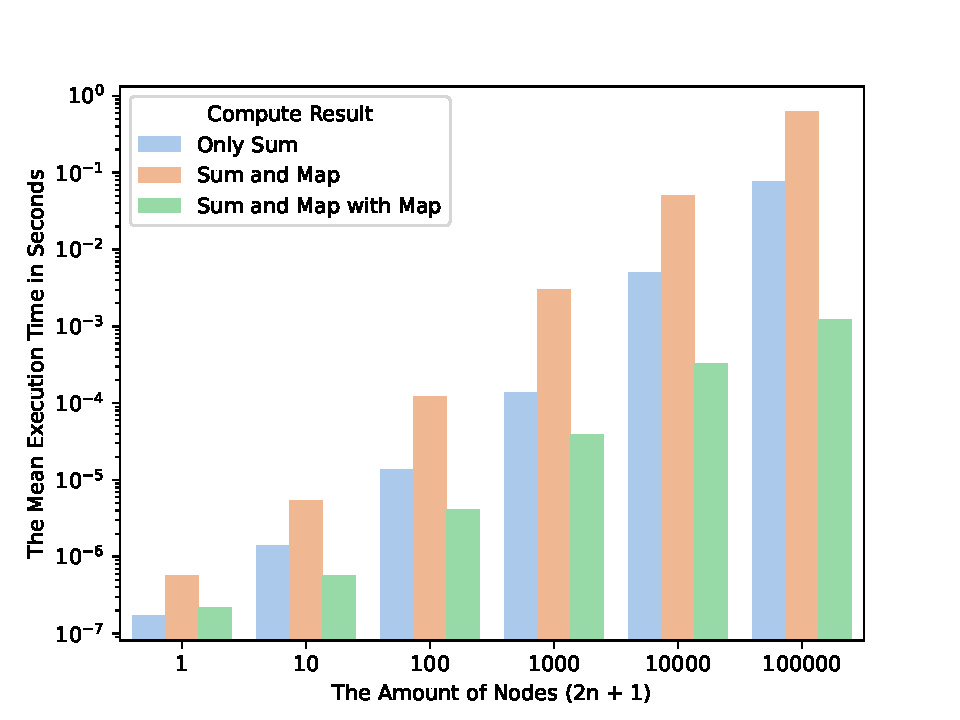
\includegraphics[width=.6\textwidth]{plot_generate_result_benchmark.pdf}
  \caption{Compute the result}
  \label{fig-compute-result}
\end{figure}